\documentclass[a4paper]{article}
\addtolength{\hoffset}
{-2.25cm}
\addtolength{\textwidth}
{5cm}
\addtolength{\voffset}
{-3.25cm}
\addtolength{\textheight}
{5.5cm}
\setlength{\parskip}{0pt}
\setlength{\parindent}{0in}

\usepackage[utf8]{inputenc}
\usepackage{microtype}
\usepackage[english]{babel}
\usepackage{fancyhdr}
\usepackage{advdate}
\usepackage{enumitem}
\usepackage{amsmath, amssymb}
\usepackage{graphicx}
\usepackage{caption}
\usepackage{subcaption}
\usepackage{float}
\usepackage{titlesec}
\usepackage{wasysym}
\usepackage{url}
\usepackage{hyperref}
\usepackage{tikz, verbatimbox}
\usepackage{fixltx2e}
\usepackage{centernot}
\usepackage{algorithm}
\usepackage{algpseudocode}
\usepackage{listings}
\usetikzlibrary{shapes.geometric, arrows}
\usetikzlibrary{positioning}
\usepackage[table]{xcolor}

\graphicspath{{./static/}}
\tikzset{every picture/.style={line width=0.75pt}} %set default line width to 0.75pt

\newcommand{\LComment}[1]{\State \(\triangleright\) \text{#1}}
\MakeRobust{\Call}
\usepackage{pdfpages}

\begin{document}

\fancyhead[c]{}
\hrule \medskip
\begin{minipage}{0.295\textwidth}
\raggedright
Rishabh Indoria\\
21F3001823
\end{minipage}
\begin{minipage}{0.4\textwidth}
\centering
\LARGE
Software Engineering
\end{minipage}
\begin{minipage}{0.295\textwidth}
\raggedleft
\today \hfill \\
\end{minipage}
\medskip \hrule
\bigskip

\section{Thinking of Software in Terms of Components}
\subsection{Case Study: Amazon System}
\begin{itemize}
    \item Components are a way of breaking the complexity of a task into manageable parts, so that different teams can work on different components of the system and put everything in a timely manner.
    \item Everyone need not the working of a component, just need to know the input and output.
    \item Amazon components: Inventory Management, Payment Gateway, Order Management, Shipping System.
    \item Inventory Management is the act of measuring the amount, location, pricing, mix of products available on Amazon.
    \item Inventory gets updated based on current purchasing and seasonal trends.
    \item Payment Gateway is a service that authorizes electronic payments.
    \item \textbf{Key Takeaway}: Software can be divided into separately addressable components called \textbf{modules} that are integrated to satisfy requirements.
    \item Amazon Pay: A mobile wallet, can link credit or debit card information, can link bank accounts, or you can transfer money online to the mobile wallet. Instead of using your debit or credit card to make purchases you can pay with your smartphone that has this mobile wallet. There are many categories like Recharges, Bill payments, Travel and Insurance, etc.
    \item First Step in create a new software component could be \textbf{study existing components of the system}, \textbf{learn a programming language}, \textbf{look at similar systems to understand features}.
    \item \textbf{Study Existing components of the system}: To understand how the new component will interact with existing components.
    \item We need to first understand what is the problem we want to solve?, and based on an analysis of existing or similar systems we need to come up with an explicit set of goals for our own system or for what our implementation should provide.
    \item \textbf{Requirements}: Goals the implemented system should have, and they should cater to the need of clients.
    \item Client can be an external user or internal users. Could be for employees or customers. Client can also be another software as well.
    \item Think about \textbf{who} is going to use your software, for \textbf{what purpose}, and in \textbf{what way}.
    \item \textbf{Key Takeaway}: Requirement specification is the first step in the software development process, through this we need to ensure that the requirements capture clients needs.
\end{itemize}

\subsection{Different phases of Development}
\begin{itemize}
    \item If we went directly to coding after specifying requirements, then we can face issues during integration where different developers may have different ideas about how the functionality should be implemented, difficulties while adding new features that is if I want to add a new feature then it would help to have a big picture view of the system.
    \item \textbf{Software Design}: Big picture view of the software system, provides a structure to the software system.
    \item When a feature is being implemented, multiple developers work together and write code for the feature, they use tools like GitHub to collaborate and write code and very often coding is done in a distributed manner with developers working in different location and even in different time zones. Hence, it is very important that everyone working on the codebase has a consistent understanding of what the code does. For this reason, all developers write \textbf{documentation} for their code and write precise interface definitions.
    \item \textbf{Interface}: An interface is the description of the actions your functions can do without describing the implementation in detail. The interface shows what requests are accepted and in what format is the corresponding response given.
    \item \textbf{Software Development}: Write code based on the requirements and the design. Usually distributed, and the developers write documentation and precise interface definitions.
    \item \textbf{Testing} is done to ensure that the software behaves according to the requirements, many bugs might still exist in the system. A failure to address bugs can even cause severe catastrophes.
    \item Testing is done at different granularities, examples include unit testing, integration testing, acceptance testing.
    \item Alpha testing done by internal employees and Beta testing done by actual users.
    \item \textbf{Maintenance}: After the feature is rolled out, monitor how users are using the feature. Purpose of doing this is to monitor what users are doing, and how they are using the software, change the code for upgrades/updates, or add features.
    \item \textbf{Overall Process}: Requirements $\rightarrow$ Design $\rightarrow$ Development $\rightarrow$ Testing $\rightarrow$ Maintenance
\end{itemize}

\subsection{Software Development Life Cycle}
\begin{itemize}
    \item \textbf{Software Lifecycle}: Different stages over which a software evolves from the initial customer request to a fully developed software.
    \item \textbf{Waterfall model}: Plan and document perspective. Each phase occurs one after the other.
    \item If we follow all phases sequentially, then the time taken could be very long, and if the client doesn't like it or has some changes we will have to start the process all over again.
    \item \textbf{Drawbacks of Waterfall}: Increase in cost, time if changes are required later on. Clients may not know what they need. Designers may not know which design might be the most feasible/usable by the clients. Can take quite long.
    \item \textbf{Prototype Model}: Build a working prototype before the development of the actual software. Prototype usually not used later.
    \item \textbf{Advantages of prototype}: Exact form of solution and technical issues are unclear, and it is useful to get feedback from customers.
    \item \textbf{Disadvantages of prototype}: Increased development costs, bugs can appear later in the development cycle.
    \item \textbf{Spiral Model}: Incrementally build the software and get feedback, refine. Combines advantages of Waterfall and Prototype model. Each iteration can still take a long time.
\end{itemize}

\subsection{Agile Perspective}
\begin{itemize}
    \item \textbf{Agile Manifesto}: Emphasizes individuals and interactions over process and tools, emphasizes over delivering working software rather than comprehensive documentation, emphasizes on customer collaboration over contract negotiation, emphasizes on responding to change over following a plan.
    \item \textbf{Incremental Development}: Teams work together to deliver the product in small increments.
    \item \textbf{Agile Approaches}: Extreme Programming(XP), Scrum(Product is built in a series of iterations known as sprints which are roughly 1–2 weeks long, this helps break done a project into several small byte sized pieces), Kanban(Software to be built is divided into small work items and these are represented on a kanban board allowing team members to see the state of any piece at any given time).
    \item \textbf{When to use Agile/Plan and Document?}: If the answer is no then Agile else Plan and Document
    \begin{itemize}
        \item Is specification required?
        \item Are customers unavailable?
        \item Is the system to be built large?
        \item Is the system to be built complex?
        \item Will it have a long product lifetime?
        \item Are you using poor software tools?
        \item Is the project team geographically distributed?
        \item Is team part of a documentation-oriented culture?
        \item Does the team have poor programming skills?
        \item Is the system to be built subject to regulation?
    \end{itemize}
    \item \href{https://www.atlassian.com/agile}{What is Agile?}
\end{itemize}


\section{Requirements Gathering and Analysis}
\subsection{Case Study: Amazon Seller Portal}
\begin{itemize}
    \item Our vision of what the software should look like and behave is quite different from what the user has in mind.
    \item We want to make sure that developers understand what customers want, customers come to an agreement about their requirements. If this does not happen we could end up with increased cost and iterations.
    \item Amazon wants to develop a portal for sellers. Products which sellers list on the portal will be available for people to buy on the Seller portal.
    \item \textbf{Primary Users}: Frequent users of the system. Example include Independent sellers, Sales team of consumer companies, Independent authors and publishers.
    \item \textbf{Secondary Users}: Do not directly use the system, use the system through an intermediary. Examples include Sales team managers.
    \item \textbf{Tertiary Users}: Do not use the software at all, affected by the introduction of the software, and Influence the purchase of the software. Examples include logistics, shipping companies, banks, people buying on Amazon.
    \item Requirements can be vague or unclear. Requirements can be inconsistent or contradicting. Requirements can be incomplete.
\end{itemize}

\subsection{Identifying Users and Requirements}
\begin{itemize}
    \item \textbf{Questionnaires}: Series of questions designed to elicit specific information from users. Good for getting answers to specific questions from a large group of people. This should be used in conjunction with other techniques.
    \item \textbf{Interviews}: Asking a set of questions, can be face-to-face, telephonic/online interviews. Can be structured, unstructured, or semi-structured. This helps to get people to explore issues, used early to elicit scenarios.
    \item \textbf{Focus Groups}: Get a group of stakeholders to discuss issues and requirements. Advantages include gaining consensus, highlighting areas of conflict, disagreement.
    \item \textbf{Naturalistic Observations}: Spending time with stakeholders as they go about their day-to-day tasks, observing their work in their natural setting. Shadowing a stakeholder, make notes, ask questions, observe.
    \item \textbf{Documentation}: Procedures and rules for a task, steps involved in an activity, regulations governing a task.
    \begin{table}[H]
        \centering
        \begin{tabular}{|c|c|}
            \hline
            \textbf{Technique} & \textbf{Good for} \\
            \hline
            Questionnaires & Answering specific questions\\
            \hline
            Interviews & Exploring issues\\
            \hline
            Focus Groups & Collecting multiple viewpoints\\
            \hline
            Naturalistic Observations & Understanding context\\
            \hline
            Documentation & Procedures, regulations, standards\\
            \hline
        \end{tabular}
    \end{table}
    \item \textbf{Basic Guidelines}: Focus on identifying stakeholders needs, involve all stakeholder groups, use combination of data gathering techniques. Run a pilot session if possible to ensure your data-gathering session is likely to go as planned.
    \item Data gathering is expensive, time-consuming - have to be pragmatic, make compromises.
    \item \textbf{Functional Requirements}: Captures a functionality required by the users from the system.
    \item \textbf{Non-Functional Requirements}: Essentially specifies how the system should behave. Examples include Reliability, Robustness, Performance, Portability, Security, etc.
    \item \textbf{Reliability}: Te extent to which a program behaves the same way over time in the same operating environment.
    \item \textbf{Robustness}: The extent to which a program can recover from errors or unexpected input.
\end{itemize}

\subsection{Software Requirement Specification}
\begin{itemize}
    \item \textbf{Requirement gathering and analysis}: Done by system analyst, along with other members of the software team. Organize these requirements in \textbf{Software Requirements Specification}(SRS) document.
    \begin{table}[H]
        \centering
        \begin{tabular}{|l|c|}
            \hline
            1. Introduction &  \\
            \hspace{1em}1.1 Purpose & \\
            \hspace{1em}1.2 Scope & \\
            \hspace{1em}1.3 Definitions, acronyms, and abbreviations & \\
            \hspace{1em}1.4 References & \\
            \hspace{1em}1.5 Overview & \\
            2. Overall Description & Broad outline and description of the software system\\
            \hspace{1em}2.1 Product Perspective & \\
            \hspace{1em}2.2 Product Functions & \\
            \hspace{1em}2.3 User Characteristics & \\
            \hspace{1em}2.4 Constrains & \\
            \hspace{1em}2.5 Assumptions and Dependencies & \\
            \hline
            3. Specific Requirements & \\
            \hspace{1em}3.1 External Interface Requirements & \\
            \hspace{2em}3.1.1 User Interfaces & \\
            \hspace{2em}3.1.2 Hardware Interfaces & \\
            \hspace{2em}3.1.3 Software Interface & \\
            \hspace{2em}3.1.4 Communication Interfaces & \\
            \hspace{1em}3.2 System Features & \\
            \hspace{2em}3.2.1 System Feature I & \\
            \hspace{3em}3.2.1.1 Introduction/Purpose of Feature & \\
            \hspace{3em}3.2.1.2 Stimulus/Response Sequence & \\
            \hspace{3em}3.2.1.3 Associated Function Requirements & Functional and Non-Functional Requirements\\
            \hspace{4em}3.2.1.3.1 Functional Requirement I & \\
            \hspace{4em}... & \\
            \hspace{4em}3.2.1.3.n Functional Requirement n & \\
            \hspace{2em}3.2.2 System Feature 2 & \\
            \hspace{2em}... & \\
            \hspace{2em}3.2.m System Feature 2 & \\
            \hspace{1em}3.3 Performance Requirements & \\
            \hspace{1em}3.4 Design Constraints & \\
            \hspace{1em}3.5 Software System Attributes & \\
            \hspace{1em}3.6 Other Requirements & \\
            \hline
        \end{tabular}
        \caption{Standard Structure of SRS document}
        \label{tab:SE-SRS-doc}
    \end{table}
    \item table \textcircled{\raisebox{-0.9pt}{\ref{tab:SE-SRS-doc}}} is a guideline of how an SRS document should look like and is not very rigid.
    \item SRS helps form an agreement between customers and developers. It helps to reduce future reworks. Provides a basis for estimating costs and schedules.
\end{itemize}

\subsection{Behavior Driven Design - User Stories}
\begin{itemize}
    \item Plan and Document perspective requires customers to be clear about their requirements before building the software, but if they are unsure of the requirements then we can follow agile perspective.
    \item \textbf{Behaviour Drive Design}: Asks questions about the behaviour of an application before and during development. Requirements are continuously refined to meet user expectations.
    \item \textbf{User Stories}: Short, Informal, plain language description of what a user wants to do within a software product which is of value of them. Smallest unit of work which can be done in 1 sprint, which is about 1–2 weeks.
    \item Role-feature-benefit pattern/template: As a [type of user], I want [an action], So that [a benefit/value].
    \begin{figure}[H]
        \centering
        \begin{subfigure}[b]{0.45\textwidth}
            \centering
            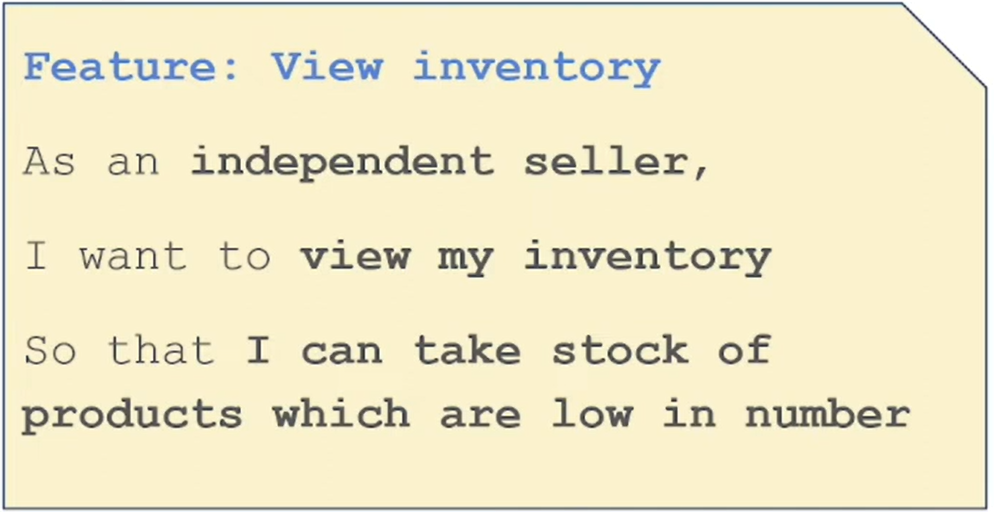
\includegraphics[width=\textwidth]{Degree/static/SE_user_story_1.png}
        \end{subfigure}
        \hfill
        \begin{subfigure}[b]{0.45\textwidth}
            \centering
            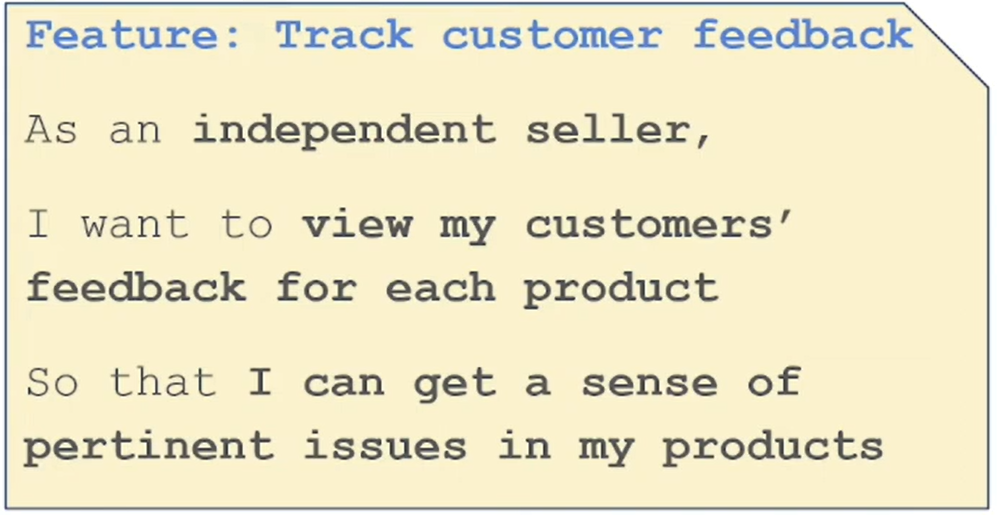
\includegraphics[width=\textwidth]{Degree/static/SE_user_story_2.png}
        \end{subfigure}
        \caption{User Story Examples}
        \label{fig:SE-user-stories}
    \end{figure}
    \item User Stories are lightweight and help plan and prioritize development. Concentrate on behaviour rather than implementation of the application. Conversation between users and the development team.
    \item \textbf{SMART}: Specific(know exactly what to implement), Measurable(known expected results for some inputs), Achievable(Implement the user story in 1-2 weeks), Relevant(Business value to one or more stakeholders), Timeboxed(Stop implementing a feature once time budget expected).
    \item May be difficult to have continuous contact with users. Not able to scale to very large projects, safety critical applications.
    \item \href{https://www.youtube.com/watch?v=KP0U3I-f9-Y}{Brief overview of the difference between requirements and user stories}.
\end{itemize}

\section{Software User Interfaces}
\subsection{Introduction to Interfaces}
\begin{itemize}
    \item Most user stories, require us to create a user interface or a UI that acts as an interaction point between the user and the software.
    \item Activities involved in Interaction Design include identifying needs and requirements, developing alternative design that meet those requirements, Build interactive versions, and Evaluate each of these designs are useful for the user.
    \item \textbf{Usability}: The extent to which a product can be used by specified end users to achieve specified goals with effectiveness, efficiency and satisfaction in a specified context of use.
    \begin{enumerate}
        \item \textbf{Effectiveness}: How good a system is at doing what it is supposed to do.Is the system capable of allowing people to learn well, carry out their work efficiently, access the information they need, buy the goods they want etc.
        \item \textbf{Efficiency}: How does a system support users in carrying out their tasks. Common tasks through minimal number of steps.
        \item \textbf{Safe to use}: Protecting the user from dangerous conditions and undesirable situations. Helping users in any situation to avoid carrying out unwanted actions accidentally.
        \item \textbf{Learnability}: How easy a system is to learn to use. Want to get started right away and carry out tasks without much effort.
        \item \textbf{Memorability}: How easy a system is to remember how to use, once learned.
    \end{enumerate}
    \item \textbf{User Experience Goals}: Want users to experience positive emotions while using the software, More subjective, How users experience a product from their perspective.
    \item \textbf{Prototypes} allow you to quickly test on users, get feedback, iterate, and pivot.
    \item Prototypes answer questions and support designers in choosing between alternatives.
    \item \textbf{Prototyping}: Test out technical feasibility of an idea, clarify some vague requirements, and User testing and evaluation.
    \item \textbf{Storyboard}: A hand drawn comic that features Setting, Sequence, and Satisfaction
    \begin{enumerate}
        \item \textbf{Setting}: People involved, Environment, Task being accomplished
        \item \textbf{Sequence}: What steps are involved? What leads someone to use the app? What task is being illustrated?
        \item \textbf{Satisfaction}: What motivates people to use the system? What does it enable people to accomplish? What need does the system fill?
    \end{enumerate}
    \item \textbf{Benefits of Storyboard}: Emphasizes how interface accomplishes a task. Avoids commitment to a particular user interface. Shared understanding among stakeholders. Some resources \href{https://www.youtube.com/watch?v=JMjozqJS44M}{video-1} and \href{https://www.youtube.com/watch?v=6dre0P4tRTc}{video-2}.
    \item \textbf{Paper Prototypes}: Hand-drawn interface on multiple pieces of paper. 
    \item \textbf{Benefits of Paper Prototypes}: Easier than writing code for user interface. Starts conversation about user interactions. Elements can be changed immediately based on given feedback.
    \item \textbf{Digital Mock-ups}: Using stuff like photoshop, PowerPoint, transform a paper prototype into a digital mockup.
    \begin{figure}[H]
        \centering
        \begin{subfigure}[b]{0.45\textwidth}
            \centering
            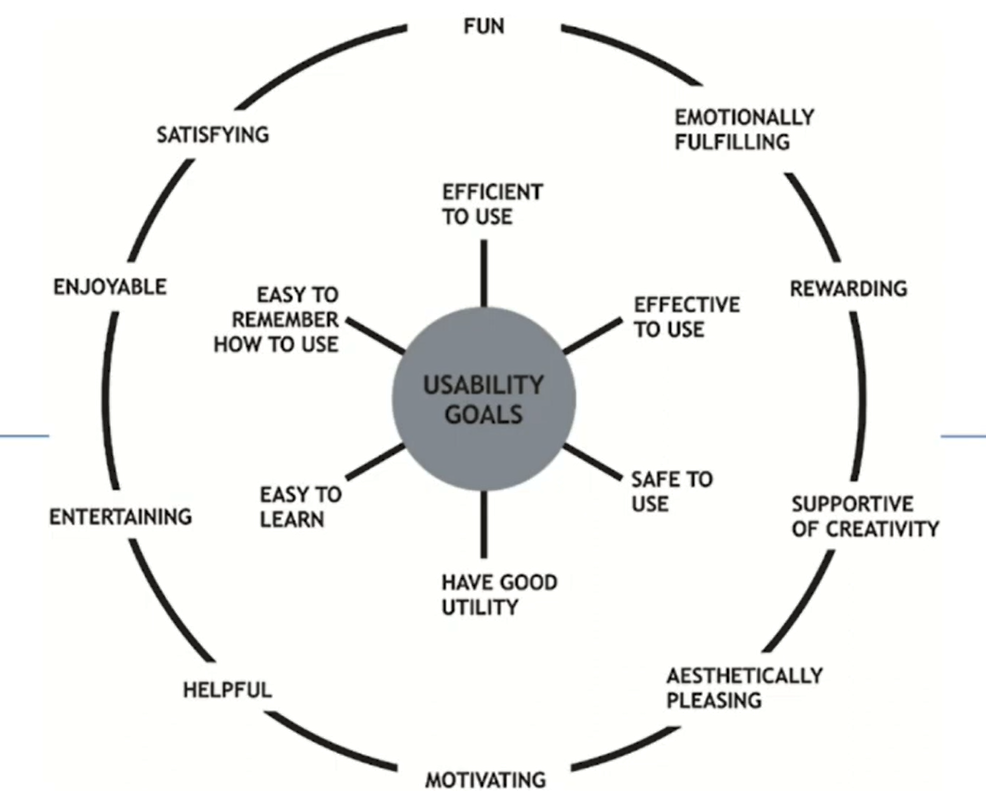
\includegraphics[width=\textwidth]{Degree//static/SE_User_Goals.png}
            \caption{User Goals Summary}
            \label{fig:SE-user-goal-summary}
        \end{subfigure}
        \hfill
        \begin{subfigure}[b]{0.45\textwidth}
            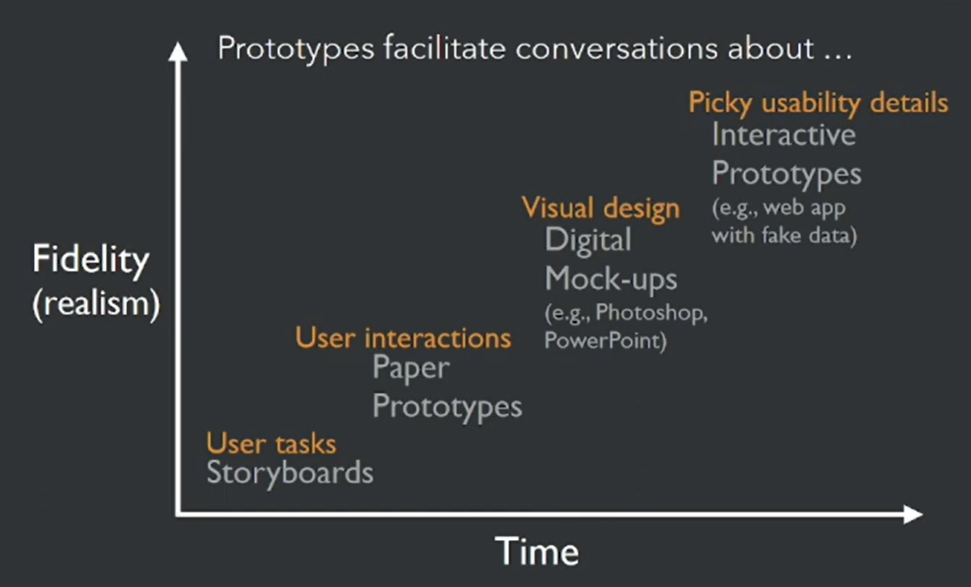
\includegraphics[width=\textwidth]{Degree/static/SE_prototype_summary.png}
            \caption{Prototypes Summary}
            \label{fig:SE-prototype-summary}
        \end{subfigure}
        \caption{Summary of Interfaces}
    \end{figure}
\end{itemize}

\subsection{Evaluation using Design Heuristics}
\begin{itemize}
    \item \textbf{Heuristic Evaluation}: Heuristics are the strategies derived from the previous experiences with similar problems. Rule of thumb/guidelines.
    \item \textbf{Heuristics for Understanding}
    \begin{enumerate}
        \item \textbf{Consistency}: Consistent Layout. Consistent Name.
        \item \textbf{Use Familiar Languages and Metaphors}
        \item \textbf{Clean and Functional Design}
    \end{enumerate}
    \item \textbf{Heuristics for Action}
    \begin{enumerate}
        \item \textbf{Freedom}: Freedom to Undo. Freedom to explore.
        \item \textbf{Flexibility}: Experts as well as new users should be able to carry out tasks efficiently.\\
        \textbf{Personalization}: Tailoring content/functionality for individual users.\\
        \textbf{Customization}: Allow users to make selections about how they want the product to work.
        \item \textbf{Recognition over Recall}: Users find it easier to recognize something they have seen earlier. Interface - buttons, navigation etc. should help the user reach his goal.
    \end{enumerate}
    \item \textbf{Heuristics for Feedback}
    \begin{enumerate}
        \item \textbf{Show Status}: Keep users informed about what is happening, through appropriate feedback within a reasonable amount of time. Provide next steps. Provide warnings in advance.
        \item \textbf{Prevent Errors}: Include helpful constraints. Offer Suggestions.
        \item \textbf{Support Error Recovery}: Make the problem clear. Provide a solution. Provide an alternate.
        \item \textbf{Provide Help}: Ensure help is easy to search. Provide help in context
    \end{enumerate}
    \item Experts evaluate the prototype, i.e., do multiple passes and provide a list of issues that violate design heuristics.
    \begin{figure}[H]
        \centering
        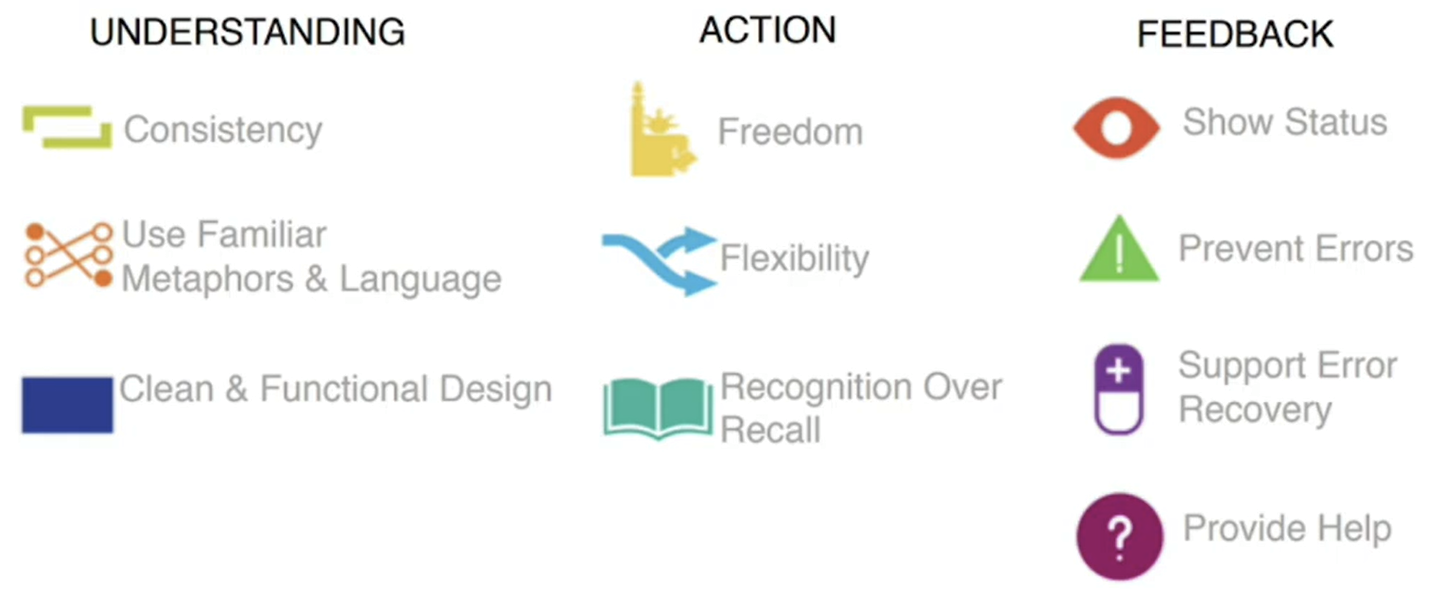
\includegraphics[width=0.5\linewidth]{Degree//static/SE_heuristic_summary.png}
        \caption{Design Heuristics Summary}
        \label{fig:ST-design-heuristic-summary}
    \end{figure}
    \item Importance of \href{https://www.vox.com/first-person/2017/3/1/14777110/typography-oscars-2017}{typography}.
\end{itemize}

\section{Project Estimation Techniques}
\subsection{Introduction}
\begin{itemize}
    \item \textbf{Importance of Estimation}: Establishing cost and Schedule. From a Client's perspective cost and schedule must be provided to them.
    \item \textbf{Key Estimation Parameters}: Size/Lines of code(KLOC, number of 1000 lines of code), Effort(How many people are required in the team, Person-month, effort an individual can typically put in a month).
    \item \textbf{Empirical Estimation}: Ask people who have completed similar projects.
    \item \textbf{Expert Judgment}: They can make an educated guess, but can encounter human errors, individual bias, optimistic estimates, overlook some factors, lack of adequate knowledge. To some extent, this can be averted by having a group of experts.
    \item \textbf{Delphi Technique}: Coordinator provides multiple Experts the SRS document and a form for recording cost estimates. Experts submit their estimates to the coordinator. Then the coordinator prepares a summary and distributes to all experts. Now, experts look at this summary and re-estimate the cost. This process can be iterated over several rounds.
    \item \textbf{Heuristic Technique}: Modelled using suitable mathematical expressions.
    \item \textbf{COCOMO Estimation Model}: Constructive Cost Estimation Model, $Effort=a\times SIZE^b$. $a$ and $b$ depend on the type of project.
    \item \textbf{Types of Projects}: Organic(Well understood application program, and team size is small and experiences), Semi-detached(Mix of experienced and inexperienced people), Embedded(Strongly couple with hardware).
    \item For Organic projects $a=2.4$ and $b=1.05$, for semi-detached project $a=3.0$ and $b=1.12$, and for embedded projects $a=3.6$ and $b=1.20$.
    \item \textbf{Effort Estimation Parameters}: People working on the project, Technical attributes of the project, Tools and practices used by the team.
    \item In COCOMO model, after getting initial estimates we add \textbf{cost driver attributes}. This would include Reliability, Database sizes, etc.
    \begin{figure}[H]
        \centering
        \begin{subfigure}[b]{0.40\textwidth}
            \centering
            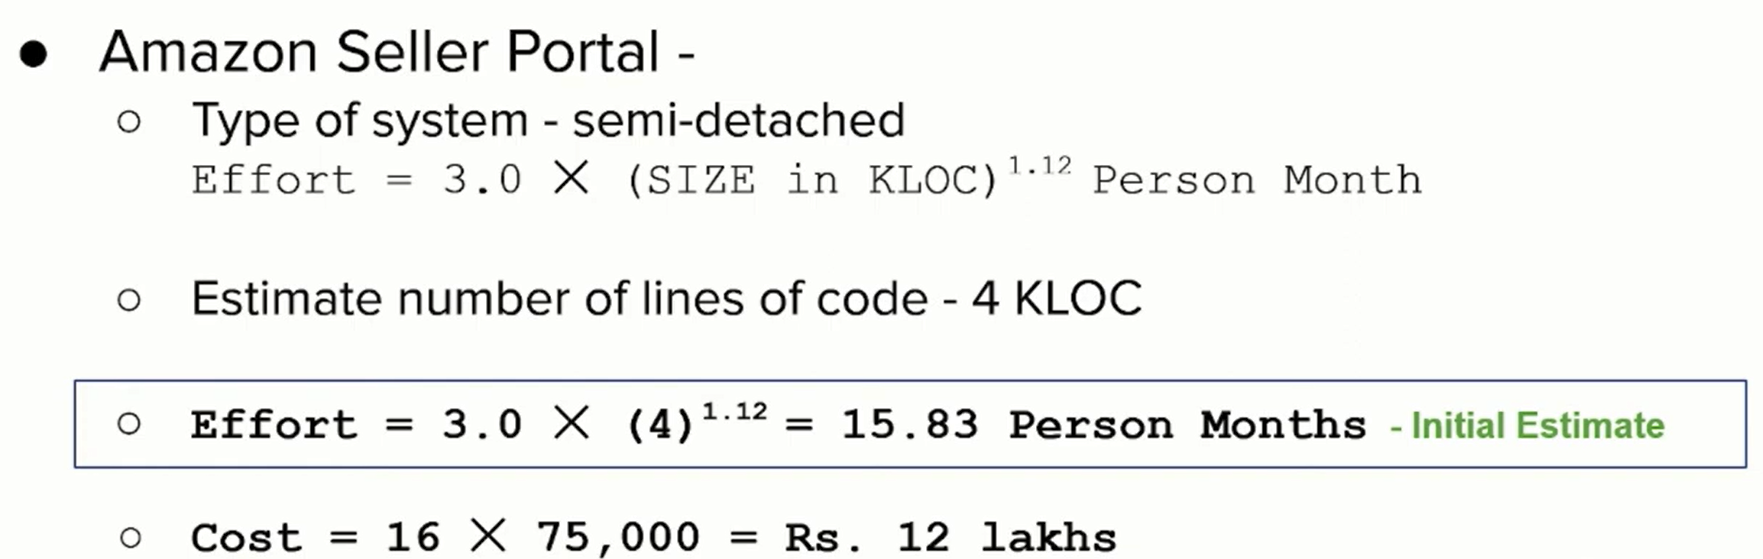
\includegraphics[width=\textwidth]{Degree/static/SE_COCOMO_ex.png}
            \caption{COCOMO model}
        \end{subfigure}
        \hfill
        \begin{subfigure}[b]{0.50\textwidth}
            \centering
            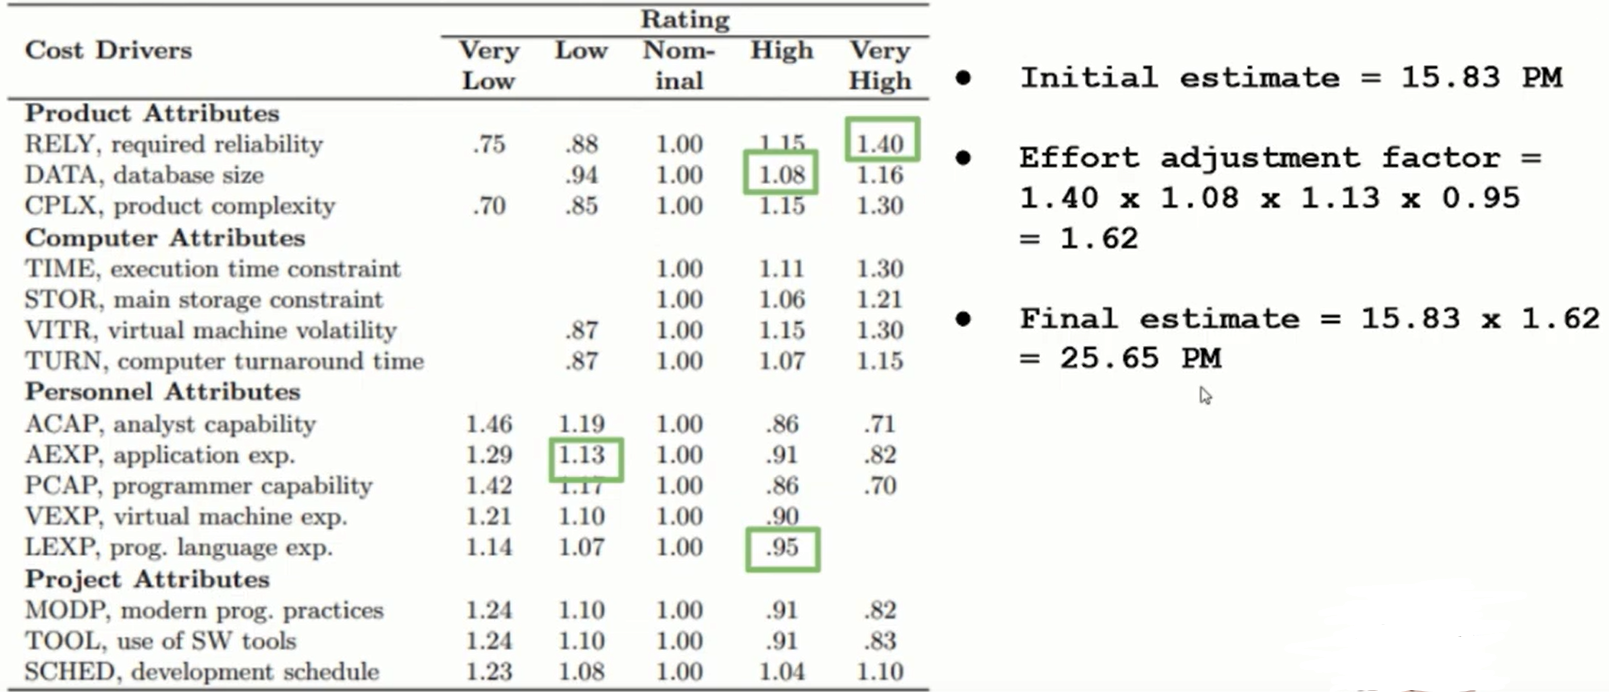
\includegraphics[width=\textwidth]{Degree/static/SE_cost_driver.png}
            \caption{Cost Drivers}
        \end{subfigure}
        \caption{Amazon Seller Portal Example}
        \label{fig:SE-amazon-seller}
    \end{figure}
\end{itemize}

\subsection{Project Scheduling}
\begin{itemize}
    \item Helps monitor timely completion of a task, and take corrective action if it falls behind.
    \item The Schedule can be built in steps as follows
    \begin{enumerate}
        \item Identify all major activities,
        \item Break down each activity into tasks,
        \item Determine the dependency among different tasks,
        \item Estimations for time durations required to complete the tasks,
        \item Represent this information in a chart/graph/network,
        \item Determine task starting and end dates from the representation,
        \item Determine the critical path(a chain of tasks that determine the duration of the project),
        \item Allocate resource to the tasks.
    \end{enumerate}
    \item Breakdown of activities can be done using \textbf{Work Breakdown Structure(WBS)}, it will create a tree like structure as follows
    \begin{enumerate}
        \item \textbf{Root}: Project name
        \item Each node is broken down into smaller activities, \textbf{children}
        \item Each leaf represents a task which can be allocated to a developer and scheduled.
        \item \textbf{Task}: Each task should take roughly two weeks to develop.
    \end{enumerate}
    \item Once we have the breakdown, now we create the activity network.
    \item \textbf{Activity Network}: Different activities making up a project, estimated durations, interdependencies. Leaf nodes of the WBS become the nodes of the activity network.
    \begin{figure}[H]
        \centering
        \begin{subfigure}[b]{0.45\textwidth}
            \centering
            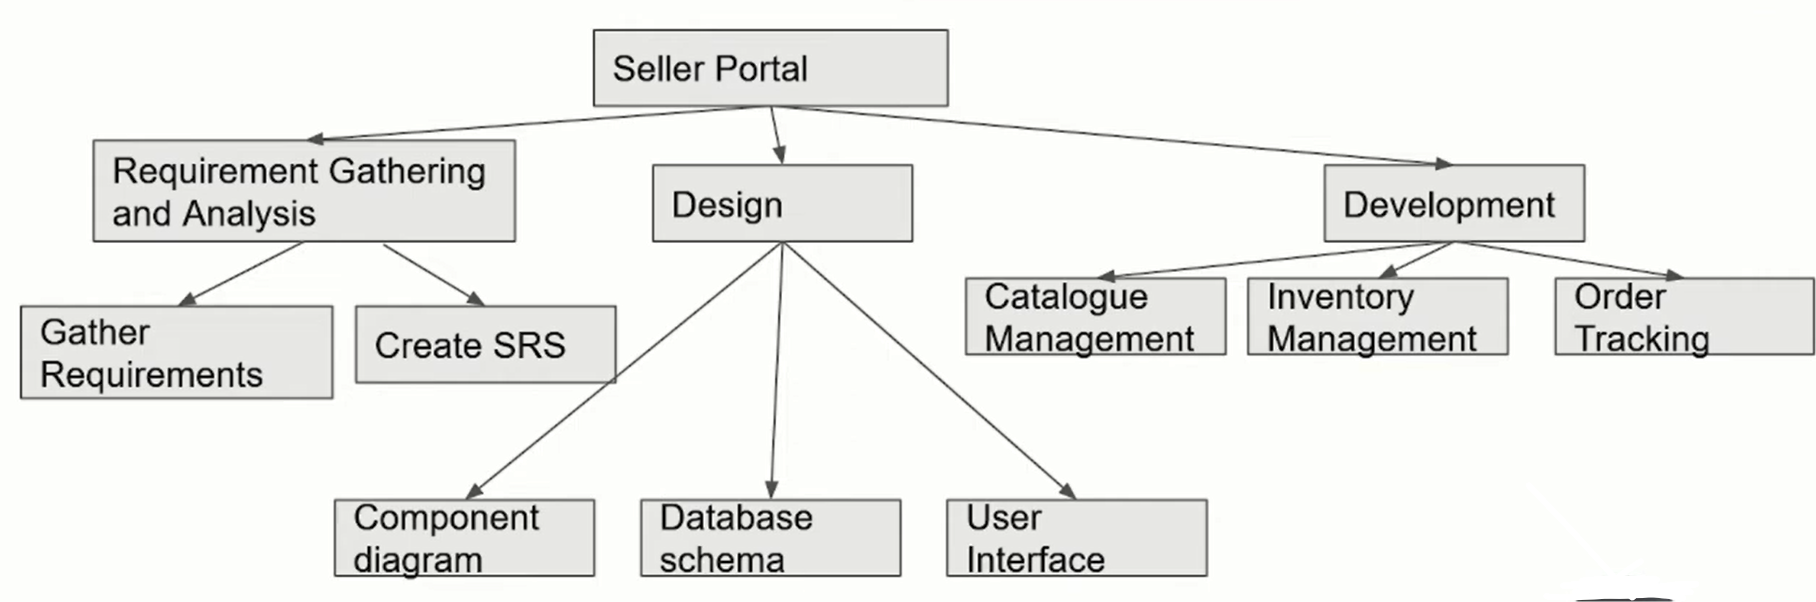
\includegraphics[width=\textwidth]{Degree/static/SE_Seller_WBS.png}
            \caption{Work Breakdown Structure}
        \end{subfigure}
        \hfill
        \begin{subfigure}[b]{0.45\textwidth}
            \centering
            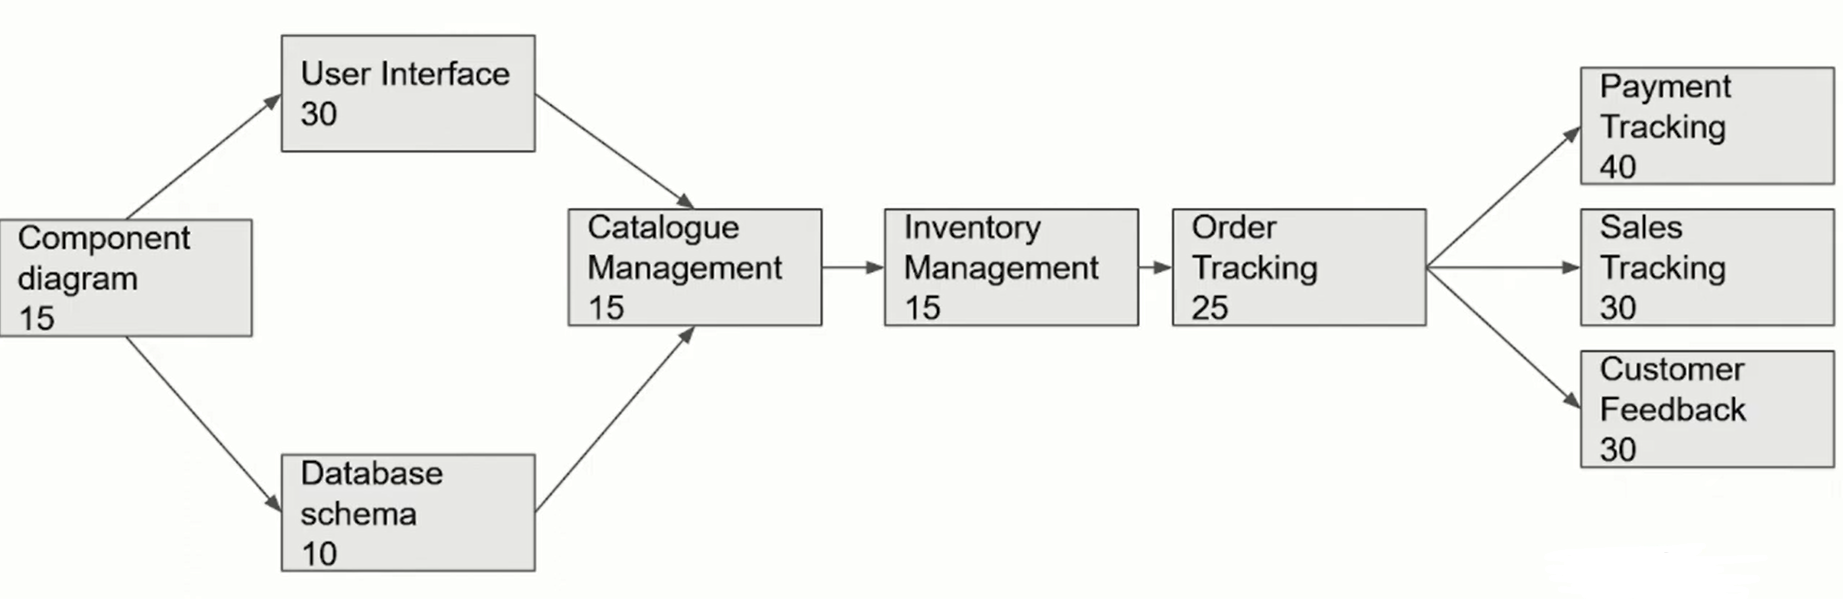
\includegraphics[width=\textwidth]{Degree/static/SE_Activity_Network.png}
            \caption{Activity Network}
        \end{subfigure}
        \caption{Seller Portal Example}
        \label{fig:SE-seller-portal}
    \end{figure}
    \item \textbf{Gantt Chart}: Another way to represent Activity network, it is a type of chart.
\end{itemize}

\subsection{Risk Management}
\begin{itemize}
    \item A risk is an anticipated unfavorable event or circumstance that can occur while a project is underway. This can be due to intangible nature of software, conflicts in a team.
    \item \textbf{Technical Risks}: Due to development team's insufficient knowledge about the product.
    \item Developing the wrong functions and user interfaces, can be mitigated by communicating with clients and build prototypes.
    \item Shortcomings in external components, can be mitigated by benchmarking and regular inspections.
    \item \textbf{Project Risks}: Project risks occur due to problems in budget, schedule, personnel, resources, and customer related problems.
    \item Most common type is schedule slippage, the project falls behind schedule, can be mitigated by creating detailed milestones, constant iterations, communicate frequently with clients.
    \item Insufficient domain knowledge/technical knowledge, can be mitigated by hiring developers with relevant experience, or we could outsource to third party vendors.
    \item Personnel shortfalls, can be mitigated by cross-training, train multiple people with skills required to work on the project.
    \item \textbf{Business Risks}: Risks which can harm the business aspects of the software product.
    \item Product is no longer competitive in the market, can be mitigated by exploring the market for similar products.
    \item Gold plating, developing unnecessary features, can be mitigated by communicating with clients and do cost-benefit analysis.
    \item \textbf{Risk Assessment}: Project manager asks everyone in the team for worst case scenario and the PM then creates a "risk table".
    \item Then a probability(P) is assigned to each risk, each risk is also assigned Impact(I), which can negligible, marginal, critical, catastrophic(1-4).
    \item The risk is then calculated as $Risk=P\times I$, which then is sorted in descending order and decide which risk need to mitigated first.
\end{itemize}

\subsection{Project Management in Agile}
\begin{itemize}
    \item Does not predict cost and schedule at the start of the project.
    \item \textbf{Team formation}: Usually team size is 4–9 people, and we organize development using \textbf{Scrum}. At the heart of scrum are sprints.
    \item \textbf{Sprint}: short, time-boxed period when a scrum team works to complete a set amount of work.
    \item \textbf{Development Team}: Whoever is required to complete work in that given sprint.
    \item \textbf{Product Owner}: Interfaces between the client and the development team.
    \item \textbf{Scrum Master}: Ensures all activities are being done well.
    \item \textbf{Sprint Planning}: This is a collaborative event between product owner, scrum master, and the development team. We ask two basic questions, What work can get done in this sprint? and How will the chosen work get done?. This meeting is roughly 2 hours per week of its iteration.
    \item \textbf{Product Backlog}: Prioritized list of work for the development team that is derived from user stories and requirements. Prioritizing will be done in sprint planning meetings.
    \item \textbf{Standup/Daily Scrum Meeting}: Daily meeting which involves everybody. Each member answers three questions, What did I work on yesterday?, What am I working on today?, and What issues are blocking me?
    \item \textbf{Sprint Review}: After the sprint the team demonstrates what they have completed. Move things from To-Do, In Progress to Done.
    \item \textbf{Sprint Retrospective}: Evaluate the last sprint, Discuss user stories/tasks that went well/didn't go well, and finally create and implement a plan.
    \item \textbf{Project Scheduling}: Key indicator of progress is how many user stories are implemented. Project estimation can be simply counting the number of user stories completed per iteration/sprint.
    \item Not all user stories require the same effort, and hence this can lead to mis-prediction. This is mitigated by assigning points to user stories, and calculate \textbf{velocity} which is the number of points per iteration/sprint.
    \item One good software to do this is \textbf{Pivotal Tracker}, Link for which can be found \href{https://www.pivotaltracker.com/}{here}.
\end{itemize}


\end{document}